\documentclass[tikz,border=2pt]{standalone}
\usepackage{amsmath,amssymb}
\usepackage{pgfplots}
\pgfplotsset{compat=1.18}
\usetikzlibrary{arrows.meta}
\begin{document}
% Compound Poisson with lambda = 3 and every claim equal to 2: S = 2N has probability
% e^{-3} 3^k / k! at s = 2k, an atom e^{-3} at zero, nothing at odd values, and mean 6.
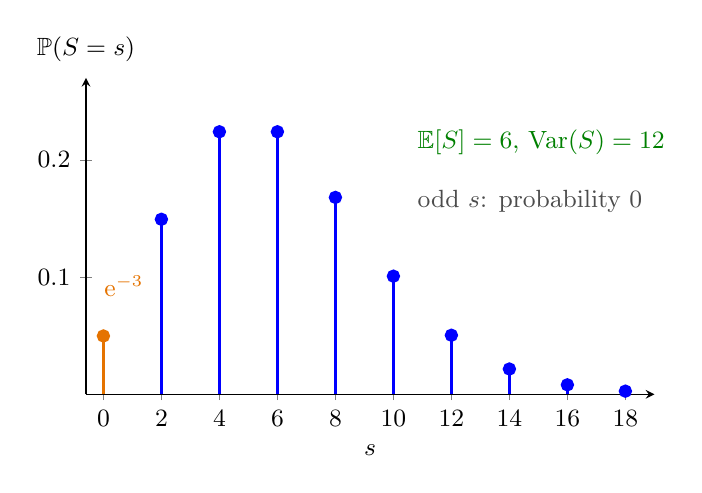
\begin{tikzpicture}[font=\small, >={Latex[length=2mm]}]
  \begin{axis}[
    axis lines=left, xmin=-0.6, xmax=19, ymin=0, ymax=0.27,
    xtick={0,2,...,18}, ytick={0.1,0.2},
    xlabel={$s$}, ylabel={$\mathbb{P}(S=s)$},
    ylabel style={rotate=-90, anchor=south, at={(axis description cs:0,1.02)}},
    width=8.8cm, height=5.6cm, clip=false]
    \addplot[blue, very thick, ycomb, mark=*, mark size=1.8pt, mark options={fill=blue}]
      coordinates {(2,0.14936) (4,0.22404) (6,0.22404) (8,0.16803) (10,0.10082) (12,0.05041) (14,0.02160) (16,0.00810) (18,0.00270)};
    \addplot[orange!90!black, very thick, ycomb, mark=*, mark size=1.8pt, mark options={fill=orange!90!black}]
      coordinates {(0,0.04979)};
    \node[orange!90!black, anchor=south west] at (axis cs:-0.3,0.075) {$\mathrm{e}^{-3}$};
    \node[green!50!black, anchor=west] at (axis cs:10.5,0.215) {$\mathbb{E}[S]=6$, $\operatorname{Var}(S)=12$};
    \node[gray!60!black, anchor=west] at (axis cs:10.5,0.165) {odd $s$: probability $0$};
  \end{axis}
\end{tikzpicture}
\end{document}
